<<<<<<< HEAD
\documentclass[
  bibliography=totoc,     % Literatur im Inhaltsverzeichnis
  captions=tableheading,  % Tabellenüberschriften
  titlepage=firstiscover, % Titelseite ist Deckblatt
]{scrartcl}

% Paket float verbessern
\usepackage{scrhack}

% Warnung, falls nochmal kompiliert werden muss
\usepackage[aux]{rerunfilecheck}

% deutsche Spracheinstellungen
\usepackage{polyglossia}
\setmainlanguage{german}

% unverzichtbare Mathe-Befehle
\usepackage{amsmath}
% viele Mathe-Symbole
\usepackage{amssymb}
% Erweiterungen für amsmath
\usepackage{mathtools}

% Fonteinstellungen
\usepackage{fontspec}
% Latin Modern Fonts werden automatisch geladen

\usepackage[
  math-style=ISO,    % ┐
  bold-style=ISO,    % │
  sans-style=italic, % │ ISO-Standard folgen
  nabla=upright,     % │
  partial=upright,   % ┘
  warnings-off={           % ┐
    mathtools-colon,       % │ unnötige Warnungen ausschalten
    mathtools-overbracket, % │
  },                       % ┘
]{unicode-math}

% traditionelle Fonts für Mathematik
\setmathfont{Latin Modern Math}
\setmathfont{XITS Math}[range={scr, bfscr}]
\setmathfont{XITS Math}[range={cal, bfcal}, StylisticSet=1]

% Zahlen und Einheiten
\usepackage[
  locale=DE,                 % deutsche Einstellungen
  separate-uncertainty=true, % immer Fehler mit \pm
  per-mode=reciprocal,       % ^-1 für inverse Einheiten
]{siunitx}

% chemische Formeln
\usepackage[
  version=4,
  math-greek=default, % ┐ mit unicode-math zusammenarbeiten
  text-greek=default, % ┘
]{mhchem}

% richtige Anführungszeichen
\usepackage[autostyle]{csquotes}

% schöne Brüche im Text
\usepackage{xfrac}

% Standardplatzierung für Floats einstellen
\usepackage{float}
\floatplacement{figure}{htbp}
\floatplacement{table}{htbp}

% Floats innerhalb einer Section halten
\usepackage[
  section, % Floats innerhalb der Section halten
  below,   % unterhalb der Section aber auf der selben Seite ist ok
]{placeins}

% Seite drehen für breite Tabellen
\usepackage{pdflscape}

% Captions schöner machen.
\usepackage[
  labelfont=bf,        % Tabelle x: Abbildung y: ist jetzt fett
  font=small,          % Schrift etwas kleiner als Dokument
  width=0.9\textwidth, % maximale Breite einer Caption schmaler
]{caption}
% subfigure, subtable, subref
\usepackage{subcaption}

% Grafiken können eingebunden werden
\usepackage{graphicx}
% größere Variation von Dateinamen möglich
\usepackage{grffile}

% schöne Tabellen
\usepackage{booktabs}

% Verbesserungen am Schriftbild
\usepackage{microtype}

% Literaturverzeichnis
\usepackage[
  backend=biber,
]{biblatex}
% Quellendatenbank
\addbibresource{lit.bib}
\addbibresource{programme.bib}

% Hyperlinks im Dokument
\usepackage[
  unicode,        % Unicode in PDF-Attributen erlauben
  pdfusetitle,    % Titel, Autoren und Datum als PDF-Attribute
  pdfcreator={},  % ┐ PDF-Attribute säubern
  pdfproducer={}, % ┘
]{hyperref}
% erweiterte Bookmarks im PDF
\usepackage{bookmark}

% Trennung von Wörtern mit Strichen
\usepackage[shortcuts]{extdash}

\author{
  Ksenia Klassen
  \texorpdfstring{
    \\
    \href{mailto:ksenia.klassen@udo.edu}{ksenia.klassen@udo.edu}
  }{}%
  \texorpdfstring{\and}{, }
  Dag-Björn Hering%
  \texorpdfstring{
    \\
    \href{mailto:dag.hering@udo.edu}{dag.hering@udo.edu}
  }{}%
}
\publishers{TU Dortmund – Fakultät Physik}

\setlength{\parindent}{0pt}%keine einrückung nach absätzen


\usepackage{longtable} 


\subject{VERSUCH NUMMER}
\title{TITEL}
\date{
  Durchführung: DATUM
  \hspace{3em}
  Abgabe: DATUM
}

\begin{document}

\maketitle
\thispagestyle{empty}
\tableofcontents
\newpage

\section{Theorie}
\label{sec:Theorie}

\cite{sample}
\subsection{Klassische Betrachtung}
Die Molwärme $C$ beschreibt die Wärmemenge $dQ$
die benötigt wird um ein Mol eines Stoffes um $dT$ zu erwärmen.
An dieser Stelle wird die spezifische Wärmekapazität bei konstantem Volumen und nicht bei
konstantem Druck unterucht.
\begin{align}
  C_{\mathrm{V}}=\frac{dQ}{dT}
\end{align}
Das Dulong-Petitsche Gesetz besagt, dass die Molwärme bei konstantem Volumen
$3R$ beträgt, mit $R$ als allgemeinen Gaskonstante, unabhängig von den Stoffeigenschaften.
Dieser Wert lässt sich durch Energiebetrachtungen am Oszillator herleiten. Da Atome in einem
festen Körper durch Gitterkräfte gebunden sind, führen diese harmonische Schwingungen
aus. Es ergibt sich schließlich der folgende Zusammenhang für die mittlere Gesammtenergie
eines Atoms:
\begin{align}
  \bigl<u\bigr>=\bigl<E_{\mathrm{kin}}\bigr>+\bigl<E_{\mathrm{pot}}\bigr>=2\bigl<E_{\mathrm{kin}}\bigr>.
\end{align}
Unter Berücksichtigung des Äquipartitionstheorems, welches besagt, dass ein Atom
pro Freiheitsgrad die mittlere kinetische Energie $\frac{1}{2}kT$ besitzt,
wenn kein Temperaturunterschied zur Umgebung herrscht, ergibt sich für
die gesamte Energie, eines auf einem Gitterplatz schwingenden Atoms, die Bezieung:
\begin{align}
  \bigl<u\bigr>=2\bigl<E_{\mathrm{kin}}\bigr>=kT.
\end{align}
Für ein Mol eines Stoffes ergibt sich mit $N_\mathrm{L}$ Atomen eine mittlere Energie von:
\begin{align}
  \bigl<U\bigr>=N_{\mathrm{L}}\bigl<u\bigr>=N_{\mathrm{L}}kT=RT
\end{align}
pro Bewegungsfreiheitsgrad.
Die Molwärme $C_{\mathrm{V}}$ hat den Dulong-Petitschen Wert:
\begin{align}
  C_{\mathrm{V}}=3R.
\end{align}\\
\subsection{Quantenmechanische Betrachtung}
Eine Problematik ergibt sich bei niedrigen Temperaturen, da wird der Molwärme Wert
von $3R$ nicht erreicht. Eine quantenmeschanische Betrachtung wird herangezogen.
Die Quantentheorie besagt, dass ein Oszillator nur Energien von bestimmter Größe
aufnehmen oder abgeben kann.
Es gilt:
\begin{align}
  \Delta u=n\cdot\hbar\cdot\omega
\end{align}
Mit weiteren Betrachtungen ergibt sich für die mittlere Energie:
\begin{align}
\bigl<U_{\mathrm{qu}}\bigr>=\frac{3N_{\mathrm{L}}\hbar\omega}{e^{\frac{\hbar\omega}{kT}}-1}.
\end{align}
Gilt $kT \gg \hbar\omega$, so strebt die Energie wieder gegen $3R$.

\section{Aufgbau und Durchführung}
\label{sec:Durchführung}
\subsection{Aufbau}
Die Messaparatur ist aufgebaut wie in Abbildung \ref{fig:aufbau}.
\begin{figure}
  \centering
  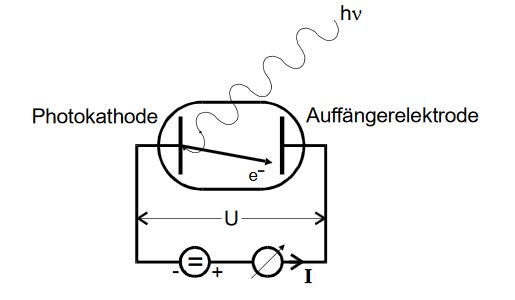
\includegraphics[width=0.6\textwidth]{aufbau.PNG}
  \caption{Aufbau der Messaparatur.}
  \label{fig:aufbau}
\end{figure}
Die im Zählrohr gesammelte Ladung fließt über den Widerstand $R$ ab und erzeugt einen Spannungsimpuls. Dieser wird über $C$ ausgekoppelt und
anschließend im Zähler registriert. Am Oszilloskop wird das Signal anschließend ausgegeben. Ein Beta-Strahler wird als Präparat
zur Messung genutzt.
\subsection{Durchführung}
Als $\beta$-Strahler wird Thallium 204 eingesetzt.
Zu Begin wird die Charakteristik aufgenommen, dazu werden verschiedene Spannungen eingestellt und die Anzahl der entsprechenden
Impulse pro $10\si{\second}$ aufgenommen. Zur Bestimmung der freigesetzten Ladungsmenge pro Teilchen, wird ebenfalls der entsprechende
Strom $I$ notiert.
Qualitativ werden die Nachentladungen auf dem Oszilloskop sichtbar gemacht. Die Spannung wird auf das Maximum gesetzt. Gemessen
wird der zeitliche Abstand von Primär-und Nachladungsimpuls. Die Totzeit lässt sich am selben
Oszillogramm gemäß Abbildung \ref{fig:tz} abmessen.
Für die Bestimmung der Totzeit mit der Zwei-Quellen-Methode werden zwei Präparate genutzt. Zuerst wird die Zählrate
des ersten Präparates aufgenommen, dann das Zweite hinzugefügt und die Zählrate der beiden gemessen. Die Zählrate nur des zweiten Präparates
wird anschließend registriert.

\section{Auswertung}
\subsection{Bestimmung der Zeitkonstante am Aufladevorgang}
\label{sec:Auswertung}
Die Messwerte zur ersten Messung finden sich in Tabelle \ref{tab:a} wieder.
Diese werden aus dem Graph aus Abbildung \ref{abb:osz} entnommen, den das Oszilloskop anzeigt. %tabelle
\begin{figure}
  \centering
  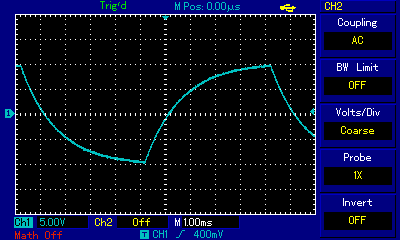
\includegraphics[width= 0.6\textwidth]{MAP001.png}
  \caption{Aufladekurve eines Kondensators über einen Widerstand}
  \label{abb:osz}
\end{figure}
\\
\\
\\
\begin{table}[h]
  \centering
  \caption{Messwerte zur Bestimmung der Zeitkonstante aus Aufladevorgang.}
  \label{tab:a}
   \begin{tabular}{c c}
     \toprule
    {$t $ \:/\: ms} & {$U_C $ \:/\: \si{\volt}}\\
    \midrule
    0.2\pm0.05 &  2.0 \pm0.05 \\
    0.4\pm0.05 &  4.2 \pm0.05 \\
    1.0\pm0.05 &  9.6 \pm0.05 \\
    1.2\pm0.05 &  11.0\pm0.05 \\
    1.4\pm0.05 &  12.2\pm0.05 \\
    1.6\pm0.05 &  13.2\pm0.05 \\
    2.0\pm0.05 &  14.8\pm0.05 \\
    2.6\pm0.05 &  16.6\pm0.05 \\
    3.0\pm0.05 &  17.4\pm0.05 \\
    3.4\pm0.05 &  18.0\pm0.05 \\
    3.8\pm0.05 &  18.4\pm0.05 \\
    4.0\pm0.05 &  18.6\pm0.05 \\
    4.4\pm0.05 &  19.0\pm0.05 \\
    4.8\pm0.05 &  19.2\pm0.05 \\
    \bottomrule
  \end{tabular}
\end{table}\\
Am Anfang wird die Formel \eqref{eqn:aufladung} in die folgegende
Form gebracht.
\begin{equation}
1-\frac{U_C}{U_0}=e^{-{\frac{1}{RC}\cdot t}}
\end{equation}
Zur Auswertung der ersten Messreihe wird der Logarithmus
von $1-\frac{U_C}{U_0}$ gegen die Zeit $t$ aufgetragen, wie in Abbildung \ref{abb:a} zu sehen.
\begin{equation}
  \ln \left(1-\frac{U_C}{U_0}\right)=-\frac{1}{RC}*t
\end{equation}
\begin{figure}[!h]
  \centering
  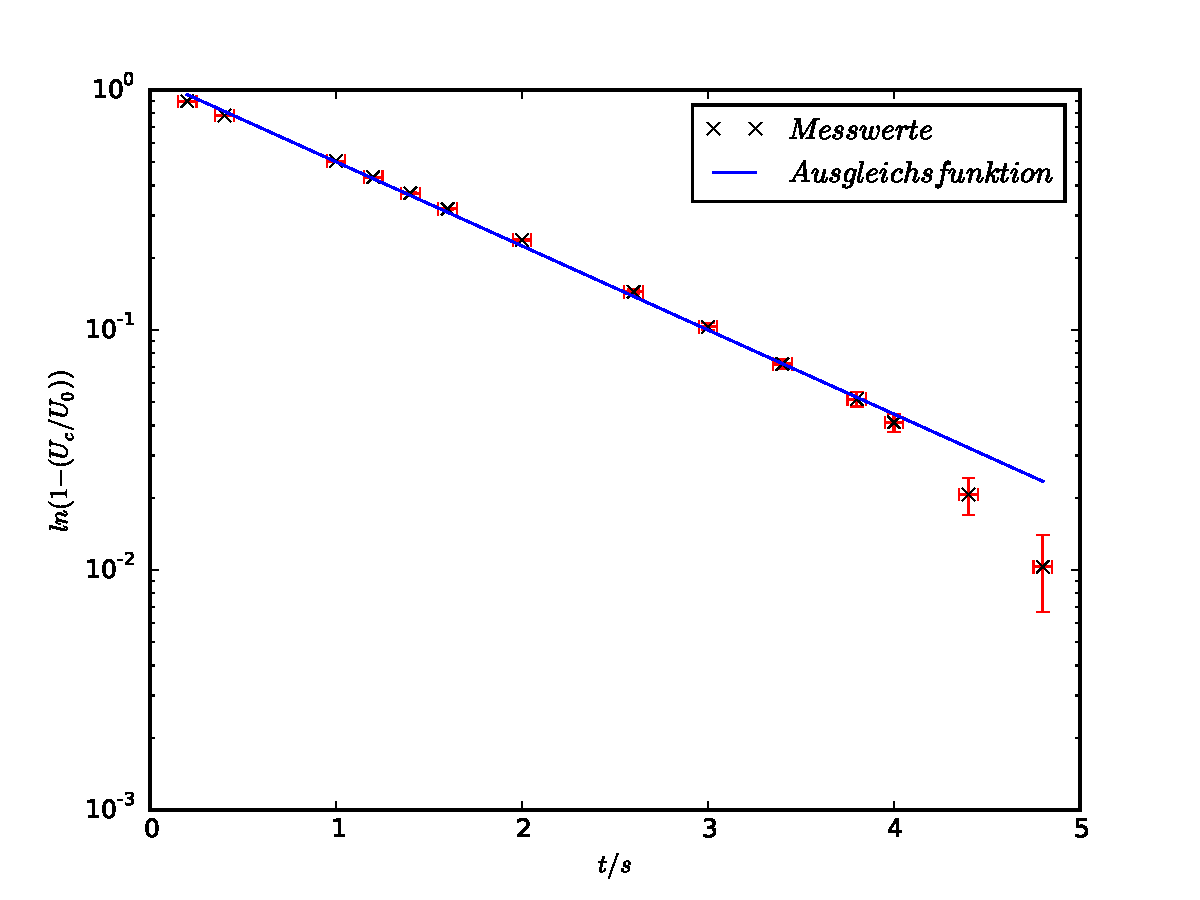
\includegraphics[width=0.7\textwidth]{a.pdf}
  \caption{Bestimmung von der $RC$-Konstant aus dem
  Aufladevorgang eines Kondensators}
\label{abb:a}
\end{figure}
\FloatBarrier
Zur Bestimmung der Zeitkonstante wird nun eine lineare Regression durchgeführt.
Das Ergebniss ist $1/RC$ als Steigung der Graden.
Der Kehrwert der Steigung ist nun die Zeitkonstante $RC$.\\
$RC$ ist hierbei:
\begin{align*}
RC_\mathrm{1}=(1,24\pm0,02)\,\si{\milli\second}
\end{align*}
\subsection{Bestimmung der Zeitkonstante mittels Frequenzabhängigkeit der Amplitude }
Erneut wird die Zeitkonstante bestimmt, nur diesmal unter
der Betrachtung von der Frequenzabhängigkeit von der Amplitude von $U_C$.
Die Amplitude wird halblogarithmisch gegen die Frequenz aufgetragen, und eine Ausgleichsrechnung
entsprechend der Gleichung \eqref{eqn:amplitude} wird durchgeführt,
diese Darstellung findet sich in Abbildung \ref{abb:b} wieder.
Die Messwerte befinden sich in Tabelle \ref{tab:b}.
Hier beträgt die Zeitkonstante
\begin{align*}
RC_\mathrm{2}=9,36 \pm 0,0007s
\end{align*}
\begin{figure}[h]
  \centering
  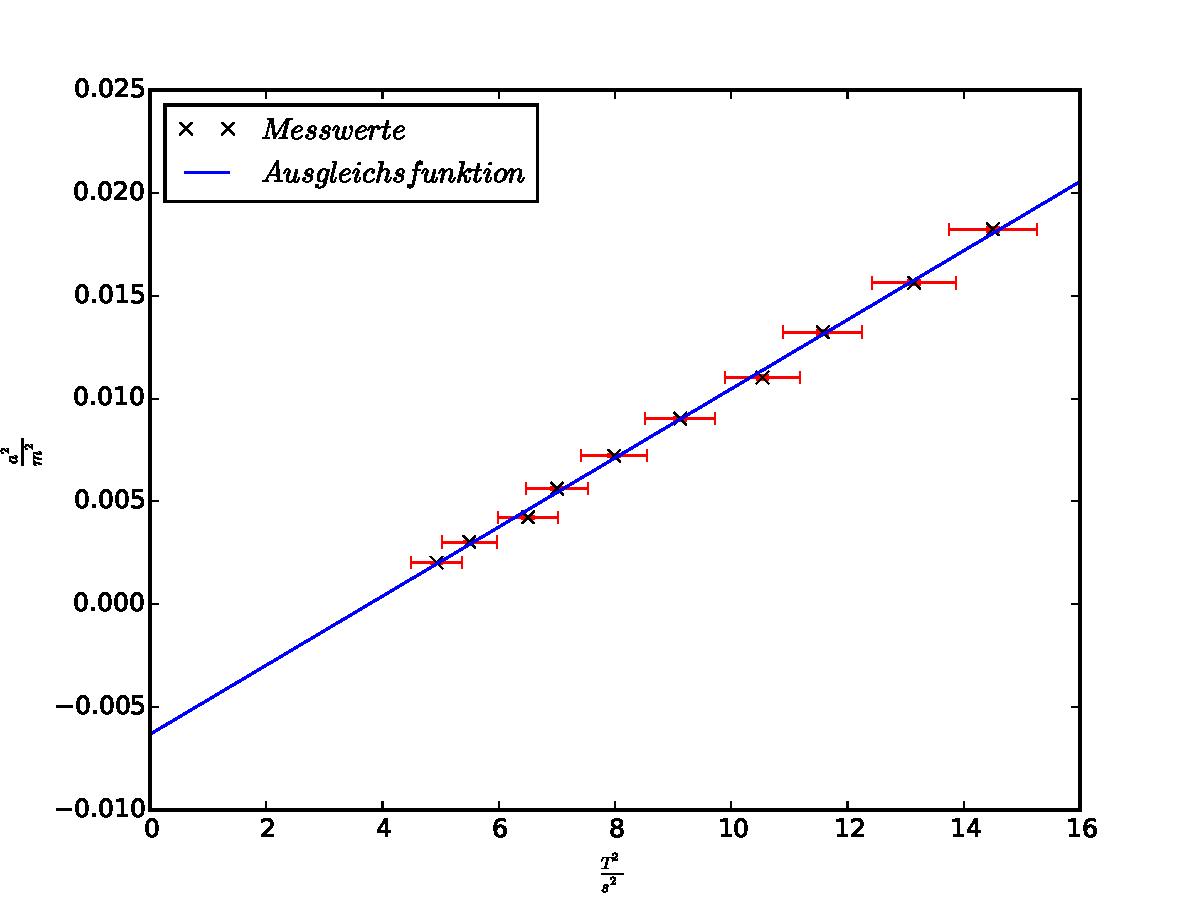
\includegraphics[width=1\textwidth]{b.pdf}
  \caption{$U_a/U_0$ in Abhängigkeit von der Frequenz $f$}
  \label{abb:b}
\end{figure}
\begin{table}[h]
  \centering
  \caption{Messwerte zur Bestimmung der Zeitkonstante aus Aufladevorgang.}
  \label{tab:b}
   \begin{tabular}{c c || c c}
     \toprule
    {$f $ \:/\: Hz} & {$A $ \:/\: \si{\volt}} & {$f $ \:/\: Hz} & {$A $ \:/\: \si{\volt}}\\
    \midrule
    50  \pm0.5 &   6.078\pm0.0005 &  1100\pm0.5 &   0.666\pm0.0005 \\
    100 \pm0.5 &   4.923\pm0.0005 &  1250\pm0.5 &   0.587\pm0.0005 \\
    150 \pm0.5 &   3.937\pm0.0005 &  1300\pm0.5 &   0.564\pm0.0005 \\
    200 \pm0.5 &   3.204\pm0.0005 &  1400\pm0.5 &   0.524\pm0.0005 \\
    250 \pm0.5 &   2.683\pm0.0005 &  1500\pm0.5 &   0.488\pm0.0005 \\
    300 \pm0.5 &   2.295\pm0.0005 &  2500\pm0.5 &   0.295\pm0.0005 \\
    350 \pm0.5 &   2.000\pm0.0005 &  3000\pm0.5 &   0.246\pm0.0005 \\
    400 \pm0.5 &   1.77 \pm0.0005 &  3500\pm0.5 &   0.211\pm0.0005 \\
    500 \pm0.5 &   1.432\pm0.0005 &  4000\pm0.5 &   0.186\pm0.0005 \\
    600 \pm0.5 &   1.202\pm0.0005 &  4500\pm0.5 &   0.166\pm0.0005 \\
    700 \pm0.5 &   1.036\pm0.0005 &  5000\pm0.5 &   0.149\pm0.0005 \\
    800 \pm0.5 &   0.91 \pm0.0005 &  6000\pm0.5 &   0.125\pm0.0005 \\
    900 \pm0.5 &   0.811\pm0.0005 &  7000\pm0.5 &   0.108\pm0.0005 \\
    950 \pm0.5 &   0.768\pm0.0005 &  10000\pm0.5 &   0.075\pm0.0005 \\
    1000\pm0.5 &   0.729\pm0.0005\\
  \bottomrule
  \end{tabular}
\end{table}
\\
\FloatBarrier
\subsection{Bestimmung der Zeitkonstante mittels Frequenzabhängigkeit der Phase}
Ein letztes Mal wird die Zeitkonstante bestimmt, diesmal mit Hilfe der Phasenverschiebung von Generator und Kondensartorspannung in Abhängigkeit von der Frequenz.
Die Werte aus Tabelle \ref{tab:c} werden gegeneinander Aufgetragen, wie in Abb.\ref{abb:c} .Die Phasenverschiebung $\phi$ wird für
die Tabelle nach Formel $\phi=\frac{a}{b}\cdot2\pi$ errechnet.
Das Ergebnis hierbei für Zeitkonstante RC ist $0.00087\pm0.0000002 s$
\begin{figure}[h]
  \centering
  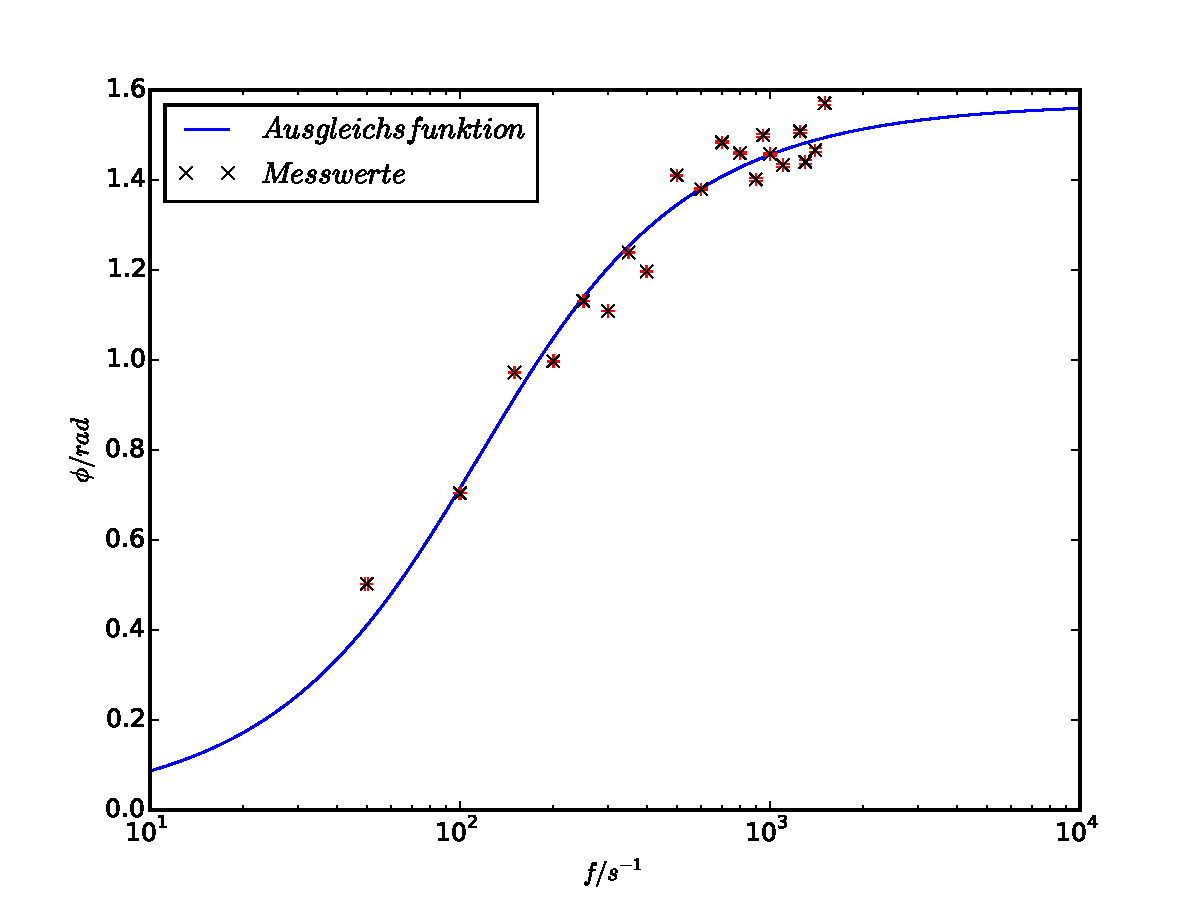
\includegraphics[width=1\textwidth]{c.pdf}
  \caption{Frequenz $f$ zur Phasenverschiebung $\phi$ aufgetragen}
  \label{abb:c}
\end{figure}
\begin{table}[h]
  \centering
  \caption{Messwerte zur Bestimmung der Zeitkonstante aus Aufladevorgang.}
  \label{tab:c}
   \begin{tabular}{c c c c}
     \toprule
    {$f $ \:/\: Hz} & {$ a $ \:/\: ms}  & {$ b $ \:/\: ms} & {$ \phi $ \:/\: $\pi$ } \\
    \midrule
    50.  \pm0.5 &  1.6  \pm0.0005 &      20. \pm0.0005   & 0.16\pm0.00005  \\
    100. \pm0.5 &  1.12 \pm0.0005 &    10.   \pm0.0005 & 0.22\pm0.0001 \\
    150. \pm0.5 &  1.04 \pm0.0005 &    6.72  \pm0.0005 & 0.31\pm0.0002 \\
    200. \pm0.5 &  0.8  \pm0.0005 &    5.04  \pm0.0005 & 0.32\pm0.0002 \\
    250. \pm0.5 &  0.72 \pm0.0005 &    4.0   \pm0.0005 & 0.35\pm0.0003 \\
    300. \pm0.5 &  0.6  \pm0.0005 &    3.4   \pm0.0005 & 0.39\pm0.0004 \\
    350. \pm0.5 &  0.56 \pm0.0005 &    2.84  \pm0.0005 & 0.38\pm0.0004 \\
    400. \pm0.5 &  0.48 \pm0.0005 &    2.52  \pm0.0005 & 0.45\pm0.0005 \\
    500. \pm0.5 &  0.44 \pm0.0005 &    1.96  \pm0.0005 & 0.44\pm0.0006 \\
    600. \pm0.5 &  0.36 \pm0.0005 &    1.64  \pm0.0005 & 0.47\pm0.0007 \\
    700. \pm0.5 &  0.34 \pm0.0005 &    1.44  \pm0.0005 & 0.46\pm0.0008 \\
    800. \pm0.5 &  0.288\pm0.0005 &    1.24  \pm0.0005 & 0.45\pm0.0009 \\
    900. \pm0.5 &  0.248\pm0.0005 &    1.112 \pm0.0005 & 0.48\pm0.001 \\
    950. \pm0.5 &  0.252\pm0.0005 &    1.056 \pm0.0005 & 0.46\pm0.001 \\
    1000.\pm0.5 &  0.232\pm0.0005 &    1.    \pm0.0005 & 0.46\pm0.001 \\
    1100.\pm0.5 &  0.208\pm0.0005 &    0.912 \pm0.0005 & 0.48\pm0.001 \\
    1250.\pm0.5 &  0.192\pm0.0005 &    0.8   \pm0.0005 & 0.46\pm0.001 \\
    1300.\pm0.5 &  0.176\pm0.0005 &    0.768 \pm0.0005 & 0.46\pm0.001 \\
    1400.\pm0.5 &  0.168\pm0.0005 &    0.72  \pm0.0005 & 0.47\pm0.001 \\
    1500.\pm0.5 &  0.168\pm0.0005 &    0.672 \pm0.0005 & 0.5\pm0.002 \\
    \bottomrule
\end{tabular}
\end{table}
\newpage
Nun werden die Werte mit identischer Frequenz
aus der Tabelle \ref{tab:b} und \ref{tab:c} in einem
Polarplott dargestellt wie in Abbildung \ref{abb:d} zu sehen.
\begin{figure}
\centering
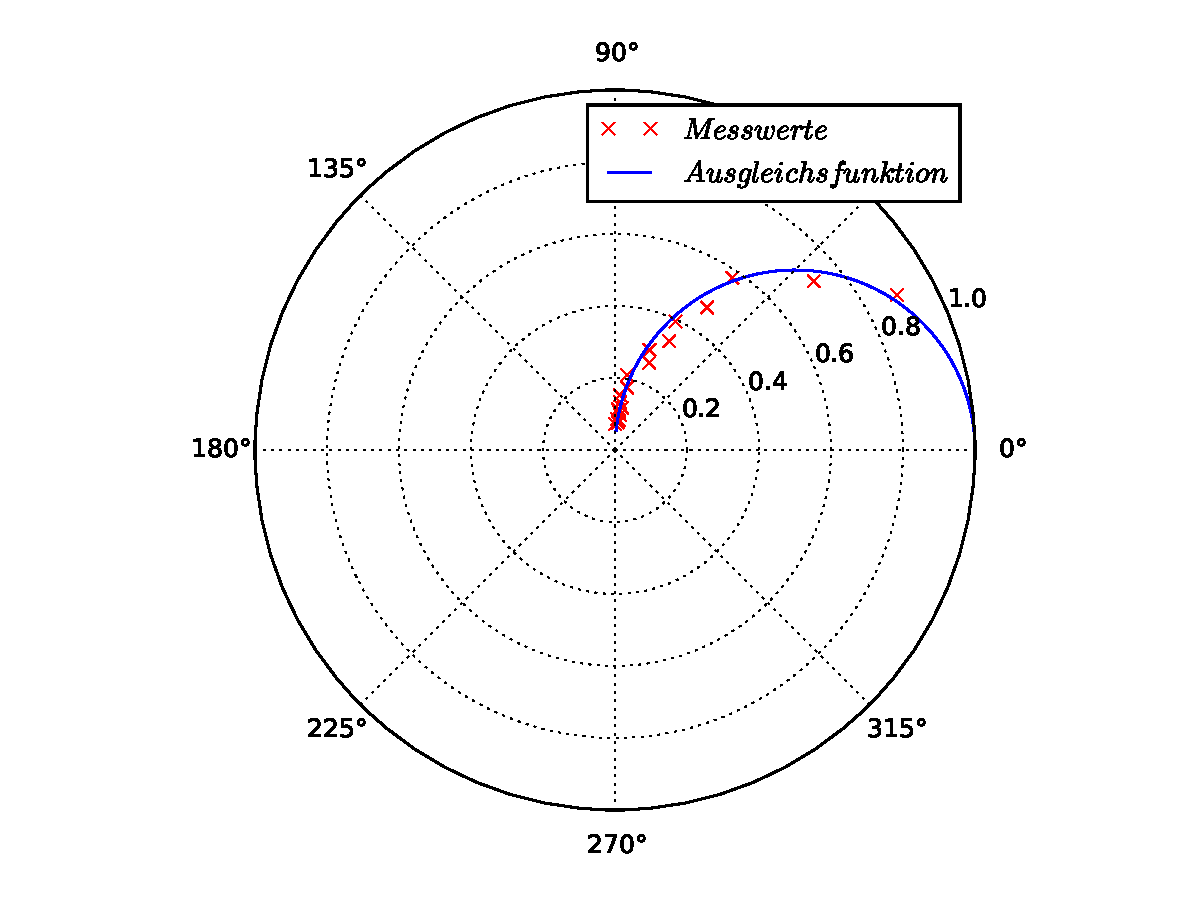
\includegraphics[width=0.8\textwidth]{d.pdf}
\caption{Amplitude $A_0$ in Abbhängigkeit von der Phasenverschiebung $\phi$ }
\label{abb:d}
\end{figure}
\FloatBarrier
\subsection{Eignung als Integrator}
Die folgenden Abbildungen zeigen die integrierten Kurven von Dreiecks-,Rechtsecks-und Sinusspannung.
Für eine Phase Sinusspannung, ergibt sich, wie in Abbildung \ref{abb:sinus} zu sehen, eine Cosinusspannung, dies entspricht auch der Stammfunktion:
\begin{align}
  f(x)&=a\cdot \sin{x}&F(x)&=-a\cdot \cos{x}.
\end{align}\\
Bei einer Phase der Rechtecksspannung ergibt sich als integrierte Spannung eine Grade mit konstanter Steigung,
zu erkennen anhand der Abbildung \ref{abb:rechteck} und der Stammfunktion:
\begin{align}
  f(x)=
  \begin{cases}
    a,& 0 \leq t \textless \pi\\
   -a,& -\pi \leq t \textless 0
  \end{cases}
  \ \ \ \ \ \ \ \ \
  F(x)=
  \begin{cases}
    a\cdot x,& 0 \leq t \textless \pi\\
   -a\cdot x,&  -\pi \leq t \textless 0.
  \end{cases}
\end{align}\\
Für eine Phase der Dreiecksspannung ergibt sich als integrierte Spannung eine Parabel, dies ist sowohl in Abbildung \ref{abb:dreieck} als auch anhand der Stammfunktion zu erkennen:
\begin{align}
  f(x)=
  \begin{cases}
    a\cdot x,& 0 \leq t \textless \pi\\
   -a\cdot x,&  -\pi \leq t \textless 0
  \end{cases}
  \ \ \ \ \ \ \ \ \
  F(x)=
  \begin{cases}
    \frac{a}{2}\cdot x^2,& 0 \leq t \textless \pi\\
   \frac{-a}{2}\cdot x^2,&  -\pi \leq t \textless 0.
  \end{cases}
\end{align}\\
\begin{figure}[h]
    \centering
    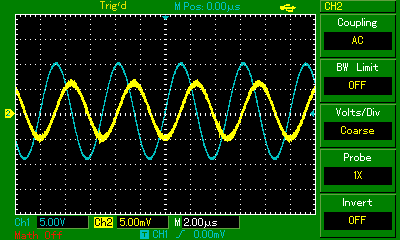
\includegraphics[width=0.6\textwidth]{MAP007.png}
    \caption{Bild der Sinusspannung und ihrer Integrierten Spannung.}
    \label{abb:sinus}
\end{figure}\\
\begin{figure}[h]
    \centering
    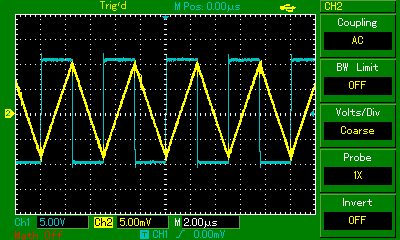
\includegraphics[width=0.6\textwidth]{MAP006.png}
    \caption{Bild der Rechteckspannung und ihrer Integrierten Spannung.}
    \label{abb:rechteck}
\end{figure}\\
\begin{figure}[h]
    \centering
    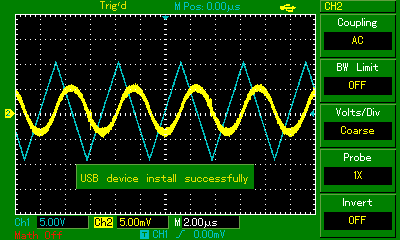
\includegraphics[width=0.6\textwidth]{MAP005.png}
    \caption{Bild der Dreicksspannung und ihrer Integrierten Spannung.}
    \label{abb:dreieck}
\end{figure}\\

\section{Diskussion}
\label{sec:Diskussion}
Nun werden die aus der Auswertung erhaltenen
Ergebnisse in Hinblick auf die Theorie untersucht.
Zu einem muss gesagt werden das die Messwerte aus der Abbildung \ref{abb:c} stark
um die Ausgleichsfunktion streuen, dies liegt daran das die Zeitabstände a und b mit
Hilfe der Cursers des Oszilloskopes gemesssen wurde und diese nicht genau eingestellt werden konnten.
Dies ließe sich mit einem Oszilloskop, das die Daten speichert und ausgibt verhmeiden.
Ebenfalls würde mit Erhöhung der Messpaare im niedrigerem Frequenzbereich die Zeitkonstant $RC$ genauer werden .
Außerdem wurde eine Frequenzabhängigkeit bei der Spannung $U_0$ gemessen, diese sank bei höheren Frequenzen ab.
Diese ist aber für den Frequenzbreich, indem die Messungen durchgeführt
worden sind, sehr gering und kann somit vernachlässigt werden.
Die bei den anderen Messverfahren erhaltenen Ergebnisse bestätigen
die aus dem Kapitel \ref{sec:Theorie} aufgeführten Formeln.


\printbibliography

\end{document}
||||||| merged common ancestors
=======
\documentclass[
  bibliography=totoc,     % Literatur im Inhaltsverzeichnis
  captions=tableheading,  % Tabellenüberschriften
  titlepage=firstiscover, % Titelseite ist Deckblatt
]{scrartcl}

% Paket float verbessern
\usepackage{scrhack}

% Warnung, falls nochmal kompiliert werden muss
\usepackage[aux]{rerunfilecheck}

% deutsche Spracheinstellungen
\usepackage{polyglossia}
\setmainlanguage{german}

% unverzichtbare Mathe-Befehle
\usepackage{amsmath}
% viele Mathe-Symbole
\usepackage{amssymb}
% Erweiterungen für amsmath
\usepackage{mathtools}

% Fonteinstellungen
\usepackage{fontspec}
% Latin Modern Fonts werden automatisch geladen

\usepackage[
  math-style=ISO,    % ┐
  bold-style=ISO,    % │
  sans-style=italic, % │ ISO-Standard folgen
  nabla=upright,     % │
  partial=upright,   % ┘
  warnings-off={           % ┐
    mathtools-colon,       % │ unnötige Warnungen ausschalten
    mathtools-overbracket, % │
  },                       % ┘
]{unicode-math}

% traditionelle Fonts für Mathematik
\setmathfont{Latin Modern Math}
\setmathfont{XITS Math}[range={scr, bfscr}]
\setmathfont{XITS Math}[range={cal, bfcal}, StylisticSet=1]

% Zahlen und Einheiten
\usepackage[
  locale=DE,                 % deutsche Einstellungen
  separate-uncertainty=true, % immer Fehler mit \pm
  per-mode=reciprocal,       % ^-1 für inverse Einheiten
]{siunitx}

% chemische Formeln
\usepackage[
  version=4,
  math-greek=default, % ┐ mit unicode-math zusammenarbeiten
  text-greek=default, % ┘
]{mhchem}

% richtige Anführungszeichen
\usepackage[autostyle]{csquotes}

% schöne Brüche im Text
\usepackage{xfrac}

% Standardplatzierung für Floats einstellen
\usepackage{float}
\floatplacement{figure}{htbp}
\floatplacement{table}{htbp}

% Floats innerhalb einer Section halten
\usepackage[
  section, % Floats innerhalb der Section halten
  below,   % unterhalb der Section aber auf der selben Seite ist ok
]{placeins}

% Seite drehen für breite Tabellen
\usepackage{pdflscape}

% Captions schöner machen.
\usepackage[
  labelfont=bf,        % Tabelle x: Abbildung y: ist jetzt fett
  font=small,          % Schrift etwas kleiner als Dokument
  width=0.9\textwidth, % maximale Breite einer Caption schmaler
]{caption}
% subfigure, subtable, subref
\usepackage{subcaption}

% Grafiken können eingebunden werden
\usepackage{graphicx}
% größere Variation von Dateinamen möglich
\usepackage{grffile}

% schöne Tabellen
\usepackage{booktabs}

% Verbesserungen am Schriftbild
\usepackage{microtype}

% Literaturverzeichnis
\usepackage[
  backend=biber,
]{biblatex}
% Quellendatenbank
\addbibresource{lit.bib}
\addbibresource{programme.bib}

% Hyperlinks im Dokument
\usepackage[
  unicode,        % Unicode in PDF-Attributen erlauben
  pdfusetitle,    % Titel, Autoren und Datum als PDF-Attribute
  pdfcreator={},  % ┐ PDF-Attribute säubern
  pdfproducer={}, % ┘
]{hyperref}
% erweiterte Bookmarks im PDF
\usepackage{bookmark}

% Trennung von Wörtern mit Strichen
\usepackage[shortcuts]{extdash}

\author{
  Ksenia Klassen
  \texorpdfstring{
    \\
    \href{mailto:ksenia.klassen@udo.edu}{ksenia.klassen@udo.edu}
  }{}%
  \texorpdfstring{\and}{, }
  Dag-Björn Hering%
  \texorpdfstring{
    \\
    \href{mailto:dag.hering@udo.edu}{dag.hering@udo.edu}
  }{}%
}
\publishers{TU Dortmund – Fakultät Physik}

\setlength{\parindent}{0pt}%keine einrückung nach absätzen


\usepackage{longtable} 


\subject{VERSUCH NUMMER}
\title{TITEL}
\date{
  Durchführung: DATUM
  \hspace{3em}
  Abgabe: DATUM
}

\begin{document}

\maketitle
\thispagestyle{empty}
\tableofcontents
\newpage
Werden Metalloberflächen erhitzt, treten Elektronen aus. Dies wird als glühelektrischer Effekt bezeichnet
und ist Gegenstaand dieses Versuchs. Untersucht werden dabei die Kennlinien und ihre drei Bereiche
einer Hochvakuumdiode.

\section{Theorie}
\label{sec:Theorie}

\cite{sample}
\subsection{Klassische Betrachtung}
Die Molwärme $C$ beschreibt die Wärmemenge $dQ$
die benötigt wird um ein Mol eines Stoffes um $dT$ zu erwärmen.
An dieser Stelle wird die spezifische Wärmekapazität bei konstantem Volumen und nicht bei
konstantem Druck unterucht.
\begin{align}
  C_{\mathrm{V}}=\frac{dQ}{dT}
\end{align}
Das Dulong-Petitsche Gesetz besagt, dass die Molwärme bei konstantem Volumen
$3R$ beträgt, mit $R$ als allgemeinen Gaskonstante, unabhängig von den Stoffeigenschaften.
Dieser Wert lässt sich durch Energiebetrachtungen am Oszillator herleiten. Da Atome in einem
festen Körper durch Gitterkräfte gebunden sind, führen diese harmonische Schwingungen
aus. Es ergibt sich schließlich der folgende Zusammenhang für die mittlere Gesammtenergie
eines Atoms:
\begin{align}
  \bigl<u\bigr>=\bigl<E_{\mathrm{kin}}\bigr>+\bigl<E_{\mathrm{pot}}\bigr>=2\bigl<E_{\mathrm{kin}}\bigr>.
\end{align}
Unter Berücksichtigung des Äquipartitionstheorems, welches besagt, dass ein Atom
pro Freiheitsgrad die mittlere kinetische Energie $\frac{1}{2}kT$ besitzt,
wenn kein Temperaturunterschied zur Umgebung herrscht, ergibt sich für
die gesamte Energie, eines auf einem Gitterplatz schwingenden Atoms, die Bezieung:
\begin{align}
  \bigl<u\bigr>=2\bigl<E_{\mathrm{kin}}\bigr>=kT.
\end{align}
Für ein Mol eines Stoffes ergibt sich mit $N_\mathrm{L}$ Atomen eine mittlere Energie von:
\begin{align}
  \bigl<U\bigr>=N_{\mathrm{L}}\bigl<u\bigr>=N_{\mathrm{L}}kT=RT
\end{align}
pro Bewegungsfreiheitsgrad.
Die Molwärme $C_{\mathrm{V}}$ hat den Dulong-Petitschen Wert:
\begin{align}
  C_{\mathrm{V}}=3R.
\end{align}\\
\subsection{Quantenmechanische Betrachtung}
Eine Problematik ergibt sich bei niedrigen Temperaturen, da wird der Molwärme Wert
von $3R$ nicht erreicht. Eine quantenmeschanische Betrachtung wird herangezogen.
Die Quantentheorie besagt, dass ein Oszillator nur Energien von bestimmter Größe
aufnehmen oder abgeben kann.
Es gilt:
\begin{align}
  \Delta u=n\cdot\hbar\cdot\omega
\end{align}
Mit weiteren Betrachtungen ergibt sich für die mittlere Energie:
\begin{align}
\bigl<U_{\mathrm{qu}}\bigr>=\frac{3N_{\mathrm{L}}\hbar\omega}{e^{\frac{\hbar\omega}{kT}}-1}.
\end{align}
Gilt $kT \gg \hbar\omega$, so strebt die Energie wieder gegen $3R$.

\section{Aufgbau und Durchführung}
\label{sec:Durchführung}
\subsection{Aufbau}
Die Messaparatur ist aufgebaut wie in Abbildung \ref{fig:aufbau}.
\begin{figure}
  \centering
  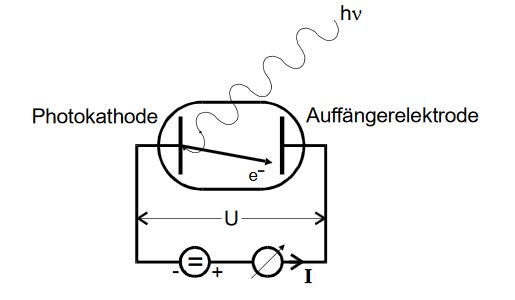
\includegraphics[width=0.6\textwidth]{aufbau.PNG}
  \caption{Aufbau der Messaparatur.}
  \label{fig:aufbau}
\end{figure}
Die im Zählrohr gesammelte Ladung fließt über den Widerstand $R$ ab und erzeugt einen Spannungsimpuls. Dieser wird über $C$ ausgekoppelt und
anschließend im Zähler registriert. Am Oszilloskop wird das Signal anschließend ausgegeben. Ein Beta-Strahler wird als Präparat
zur Messung genutzt.
\subsection{Durchführung}
Als $\beta$-Strahler wird Thallium 204 eingesetzt.
Zu Begin wird die Charakteristik aufgenommen, dazu werden verschiedene Spannungen eingestellt und die Anzahl der entsprechenden
Impulse pro $10\si{\second}$ aufgenommen. Zur Bestimmung der freigesetzten Ladungsmenge pro Teilchen, wird ebenfalls der entsprechende
Strom $I$ notiert.
Qualitativ werden die Nachentladungen auf dem Oszilloskop sichtbar gemacht. Die Spannung wird auf das Maximum gesetzt. Gemessen
wird der zeitliche Abstand von Primär-und Nachladungsimpuls. Die Totzeit lässt sich am selben
Oszillogramm gemäß Abbildung \ref{fig:tz} abmessen.
Für die Bestimmung der Totzeit mit der Zwei-Quellen-Methode werden zwei Präparate genutzt. Zuerst wird die Zählrate
des ersten Präparates aufgenommen, dann das Zweite hinzugefügt und die Zählrate der beiden gemessen. Die Zählrate nur des zweiten Präparates
wird anschließend registriert.

\section{Auswertung}
\subsection{Bestimmung der Zeitkonstante am Aufladevorgang}
\label{sec:Auswertung}
Die Messwerte zur ersten Messung finden sich in Tabelle \ref{tab:a} wieder.
Diese werden aus dem Graph aus Abbildung \ref{abb:osz} entnommen, den das Oszilloskop anzeigt. %tabelle
\begin{figure}
  \centering
  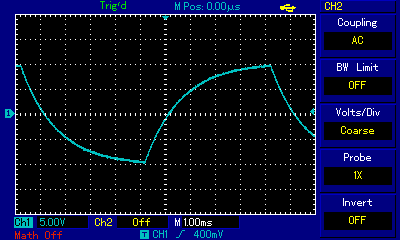
\includegraphics[width= 0.6\textwidth]{MAP001.png}
  \caption{Aufladekurve eines Kondensators über einen Widerstand}
  \label{abb:osz}
\end{figure}
\\
\\
\\
\begin{table}[h]
  \centering
  \caption{Messwerte zur Bestimmung der Zeitkonstante aus Aufladevorgang.}
  \label{tab:a}
   \begin{tabular}{c c}
     \toprule
    {$t $ \:/\: ms} & {$U_C $ \:/\: \si{\volt}}\\
    \midrule
    0.2\pm0.05 &  2.0 \pm0.05 \\
    0.4\pm0.05 &  4.2 \pm0.05 \\
    1.0\pm0.05 &  9.6 \pm0.05 \\
    1.2\pm0.05 &  11.0\pm0.05 \\
    1.4\pm0.05 &  12.2\pm0.05 \\
    1.6\pm0.05 &  13.2\pm0.05 \\
    2.0\pm0.05 &  14.8\pm0.05 \\
    2.6\pm0.05 &  16.6\pm0.05 \\
    3.0\pm0.05 &  17.4\pm0.05 \\
    3.4\pm0.05 &  18.0\pm0.05 \\
    3.8\pm0.05 &  18.4\pm0.05 \\
    4.0\pm0.05 &  18.6\pm0.05 \\
    4.4\pm0.05 &  19.0\pm0.05 \\
    4.8\pm0.05 &  19.2\pm0.05 \\
    \bottomrule
  \end{tabular}
\end{table}\\
Am Anfang wird die Formel \eqref{eqn:aufladung} in die folgegende
Form gebracht.
\begin{equation}
1-\frac{U_C}{U_0}=e^{-{\frac{1}{RC}\cdot t}}
\end{equation}
Zur Auswertung der ersten Messreihe wird der Logarithmus
von $1-\frac{U_C}{U_0}$ gegen die Zeit $t$ aufgetragen, wie in Abbildung \ref{abb:a} zu sehen.
\begin{equation}
  \ln \left(1-\frac{U_C}{U_0}\right)=-\frac{1}{RC}*t
\end{equation}
\begin{figure}[!h]
  \centering
  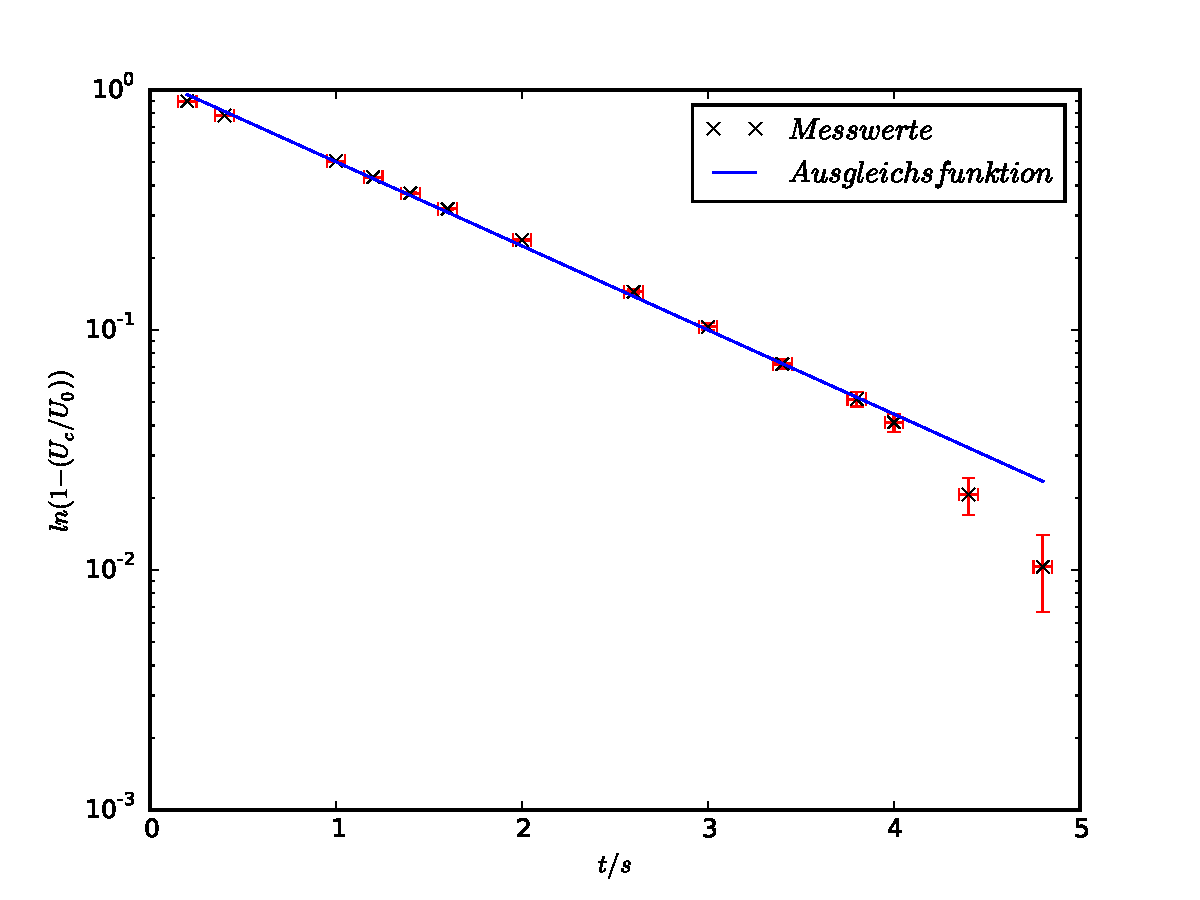
\includegraphics[width=0.7\textwidth]{a.pdf}
  \caption{Bestimmung von der $RC$-Konstant aus dem
  Aufladevorgang eines Kondensators}
\label{abb:a}
\end{figure}
\FloatBarrier
Zur Bestimmung der Zeitkonstante wird nun eine lineare Regression durchgeführt.
Das Ergebniss ist $1/RC$ als Steigung der Graden.
Der Kehrwert der Steigung ist nun die Zeitkonstante $RC$.\\
$RC$ ist hierbei:
\begin{align*}
RC_\mathrm{1}=(1,24\pm0,02)\,\si{\milli\second}
\end{align*}
\subsection{Bestimmung der Zeitkonstante mittels Frequenzabhängigkeit der Amplitude }
Erneut wird die Zeitkonstante bestimmt, nur diesmal unter
der Betrachtung von der Frequenzabhängigkeit von der Amplitude von $U_C$.
Die Amplitude wird halblogarithmisch gegen die Frequenz aufgetragen, und eine Ausgleichsrechnung
entsprechend der Gleichung \eqref{eqn:amplitude} wird durchgeführt,
diese Darstellung findet sich in Abbildung \ref{abb:b} wieder.
Die Messwerte befinden sich in Tabelle \ref{tab:b}.
Hier beträgt die Zeitkonstante
\begin{align*}
RC_\mathrm{2}=9,36 \pm 0,0007s
\end{align*}
\begin{figure}[h]
  \centering
  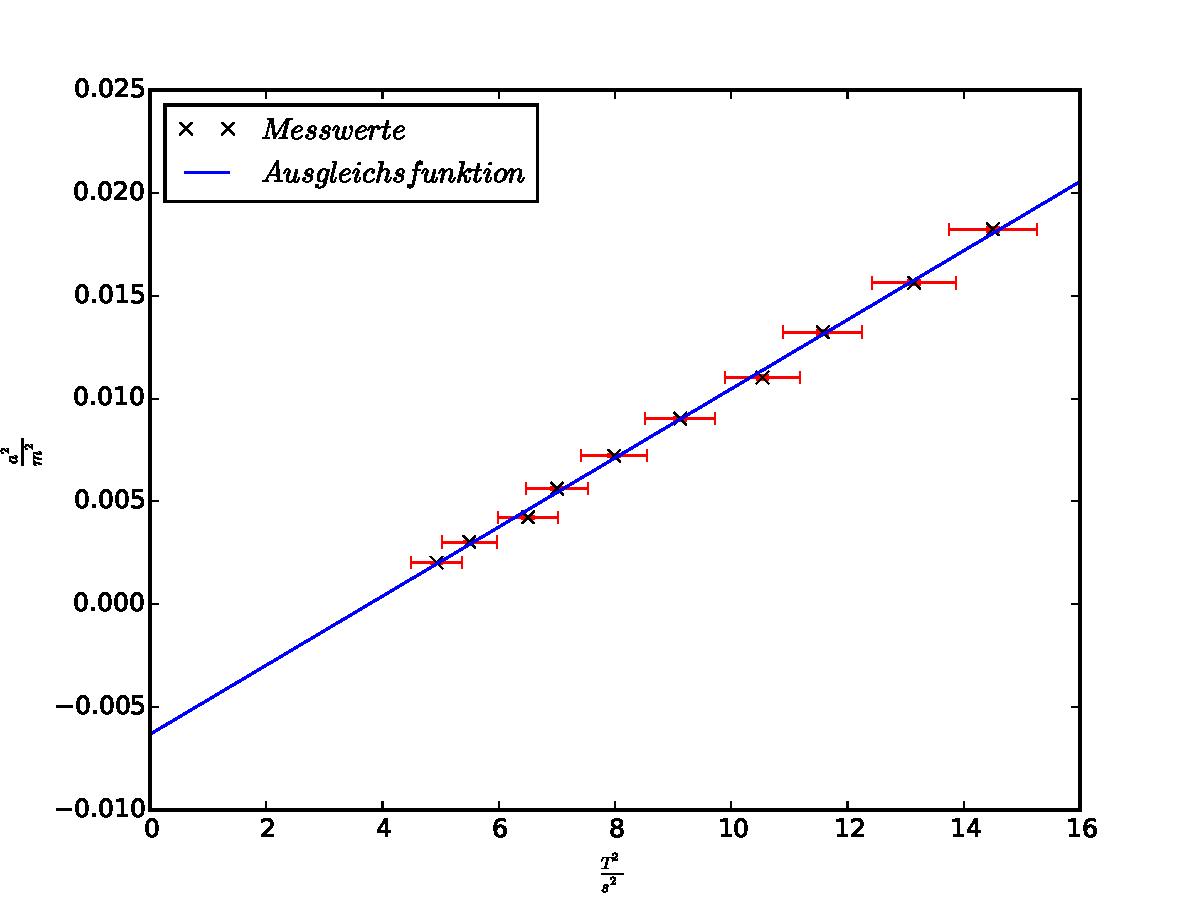
\includegraphics[width=1\textwidth]{b.pdf}
  \caption{$U_a/U_0$ in Abhängigkeit von der Frequenz $f$}
  \label{abb:b}
\end{figure}
\begin{table}[h]
  \centering
  \caption{Messwerte zur Bestimmung der Zeitkonstante aus Aufladevorgang.}
  \label{tab:b}
   \begin{tabular}{c c || c c}
     \toprule
    {$f $ \:/\: Hz} & {$A $ \:/\: \si{\volt}} & {$f $ \:/\: Hz} & {$A $ \:/\: \si{\volt}}\\
    \midrule
    50  \pm0.5 &   6.078\pm0.0005 &  1100\pm0.5 &   0.666\pm0.0005 \\
    100 \pm0.5 &   4.923\pm0.0005 &  1250\pm0.5 &   0.587\pm0.0005 \\
    150 \pm0.5 &   3.937\pm0.0005 &  1300\pm0.5 &   0.564\pm0.0005 \\
    200 \pm0.5 &   3.204\pm0.0005 &  1400\pm0.5 &   0.524\pm0.0005 \\
    250 \pm0.5 &   2.683\pm0.0005 &  1500\pm0.5 &   0.488\pm0.0005 \\
    300 \pm0.5 &   2.295\pm0.0005 &  2500\pm0.5 &   0.295\pm0.0005 \\
    350 \pm0.5 &   2.000\pm0.0005 &  3000\pm0.5 &   0.246\pm0.0005 \\
    400 \pm0.5 &   1.77 \pm0.0005 &  3500\pm0.5 &   0.211\pm0.0005 \\
    500 \pm0.5 &   1.432\pm0.0005 &  4000\pm0.5 &   0.186\pm0.0005 \\
    600 \pm0.5 &   1.202\pm0.0005 &  4500\pm0.5 &   0.166\pm0.0005 \\
    700 \pm0.5 &   1.036\pm0.0005 &  5000\pm0.5 &   0.149\pm0.0005 \\
    800 \pm0.5 &   0.91 \pm0.0005 &  6000\pm0.5 &   0.125\pm0.0005 \\
    900 \pm0.5 &   0.811\pm0.0005 &  7000\pm0.5 &   0.108\pm0.0005 \\
    950 \pm0.5 &   0.768\pm0.0005 &  10000\pm0.5 &   0.075\pm0.0005 \\
    1000\pm0.5 &   0.729\pm0.0005\\
  \bottomrule
  \end{tabular}
\end{table}
\\
\FloatBarrier
\subsection{Bestimmung der Zeitkonstante mittels Frequenzabhängigkeit der Phase}
Ein letztes Mal wird die Zeitkonstante bestimmt, diesmal mit Hilfe der Phasenverschiebung von Generator und Kondensartorspannung in Abhängigkeit von der Frequenz.
Die Werte aus Tabelle \ref{tab:c} werden gegeneinander Aufgetragen, wie in Abb.\ref{abb:c} .Die Phasenverschiebung $\phi$ wird für
die Tabelle nach Formel $\phi=\frac{a}{b}\cdot2\pi$ errechnet.
Das Ergebnis hierbei für Zeitkonstante RC ist $0.00087\pm0.0000002 s$
\begin{figure}[h]
  \centering
  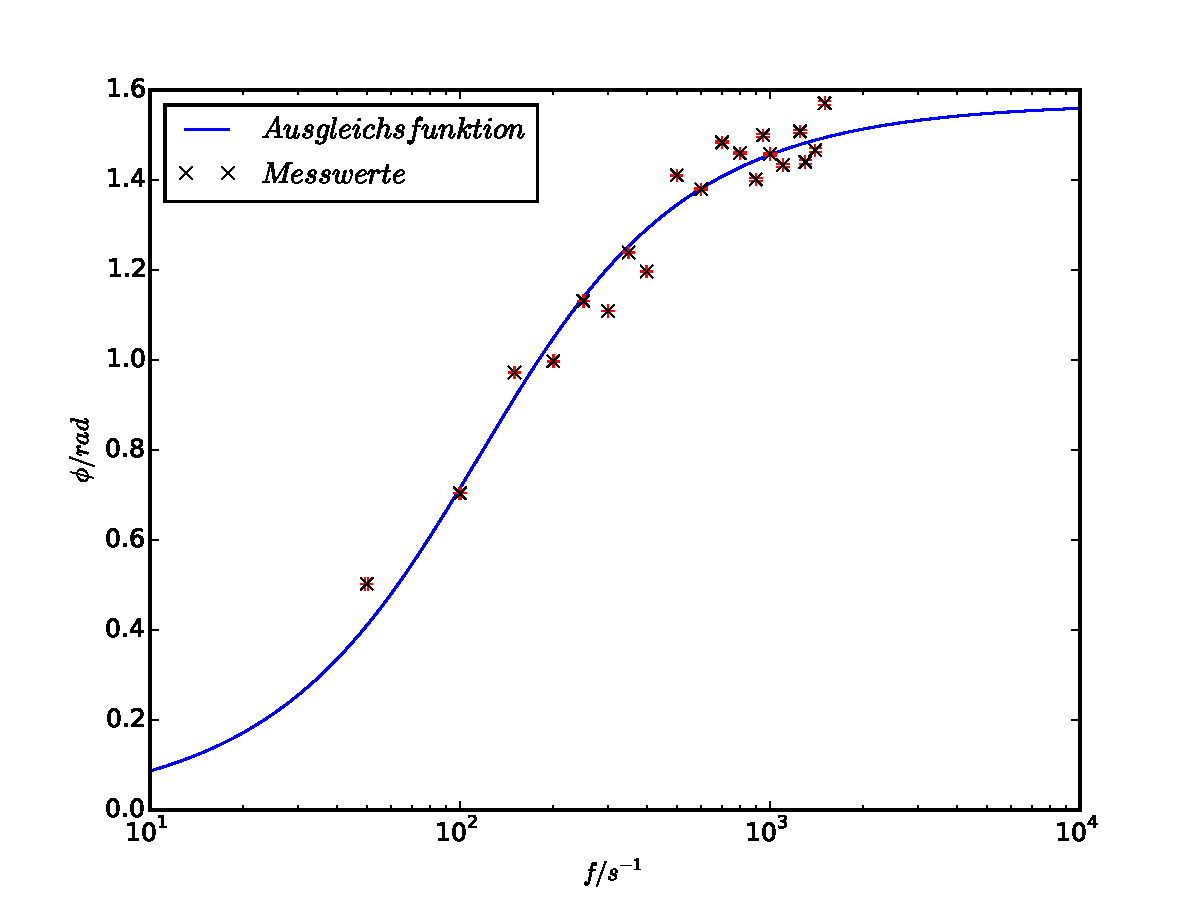
\includegraphics[width=1\textwidth]{c.pdf}
  \caption{Frequenz $f$ zur Phasenverschiebung $\phi$ aufgetragen}
  \label{abb:c}
\end{figure}
\begin{table}[h]
  \centering
  \caption{Messwerte zur Bestimmung der Zeitkonstante aus Aufladevorgang.}
  \label{tab:c}
   \begin{tabular}{c c c c}
     \toprule
    {$f $ \:/\: Hz} & {$ a $ \:/\: ms}  & {$ b $ \:/\: ms} & {$ \phi $ \:/\: $\pi$ } \\
    \midrule
    50.  \pm0.5 &  1.6  \pm0.0005 &      20. \pm0.0005   & 0.16\pm0.00005  \\
    100. \pm0.5 &  1.12 \pm0.0005 &    10.   \pm0.0005 & 0.22\pm0.0001 \\
    150. \pm0.5 &  1.04 \pm0.0005 &    6.72  \pm0.0005 & 0.31\pm0.0002 \\
    200. \pm0.5 &  0.8  \pm0.0005 &    5.04  \pm0.0005 & 0.32\pm0.0002 \\
    250. \pm0.5 &  0.72 \pm0.0005 &    4.0   \pm0.0005 & 0.35\pm0.0003 \\
    300. \pm0.5 &  0.6  \pm0.0005 &    3.4   \pm0.0005 & 0.39\pm0.0004 \\
    350. \pm0.5 &  0.56 \pm0.0005 &    2.84  \pm0.0005 & 0.38\pm0.0004 \\
    400. \pm0.5 &  0.48 \pm0.0005 &    2.52  \pm0.0005 & 0.45\pm0.0005 \\
    500. \pm0.5 &  0.44 \pm0.0005 &    1.96  \pm0.0005 & 0.44\pm0.0006 \\
    600. \pm0.5 &  0.36 \pm0.0005 &    1.64  \pm0.0005 & 0.47\pm0.0007 \\
    700. \pm0.5 &  0.34 \pm0.0005 &    1.44  \pm0.0005 & 0.46\pm0.0008 \\
    800. \pm0.5 &  0.288\pm0.0005 &    1.24  \pm0.0005 & 0.45\pm0.0009 \\
    900. \pm0.5 &  0.248\pm0.0005 &    1.112 \pm0.0005 & 0.48\pm0.001 \\
    950. \pm0.5 &  0.252\pm0.0005 &    1.056 \pm0.0005 & 0.46\pm0.001 \\
    1000.\pm0.5 &  0.232\pm0.0005 &    1.    \pm0.0005 & 0.46\pm0.001 \\
    1100.\pm0.5 &  0.208\pm0.0005 &    0.912 \pm0.0005 & 0.48\pm0.001 \\
    1250.\pm0.5 &  0.192\pm0.0005 &    0.8   \pm0.0005 & 0.46\pm0.001 \\
    1300.\pm0.5 &  0.176\pm0.0005 &    0.768 \pm0.0005 & 0.46\pm0.001 \\
    1400.\pm0.5 &  0.168\pm0.0005 &    0.72  \pm0.0005 & 0.47\pm0.001 \\
    1500.\pm0.5 &  0.168\pm0.0005 &    0.672 \pm0.0005 & 0.5\pm0.002 \\
    \bottomrule
\end{tabular}
\end{table}
\newpage
Nun werden die Werte mit identischer Frequenz
aus der Tabelle \ref{tab:b} und \ref{tab:c} in einem
Polarplott dargestellt wie in Abbildung \ref{abb:d} zu sehen.
\begin{figure}
\centering
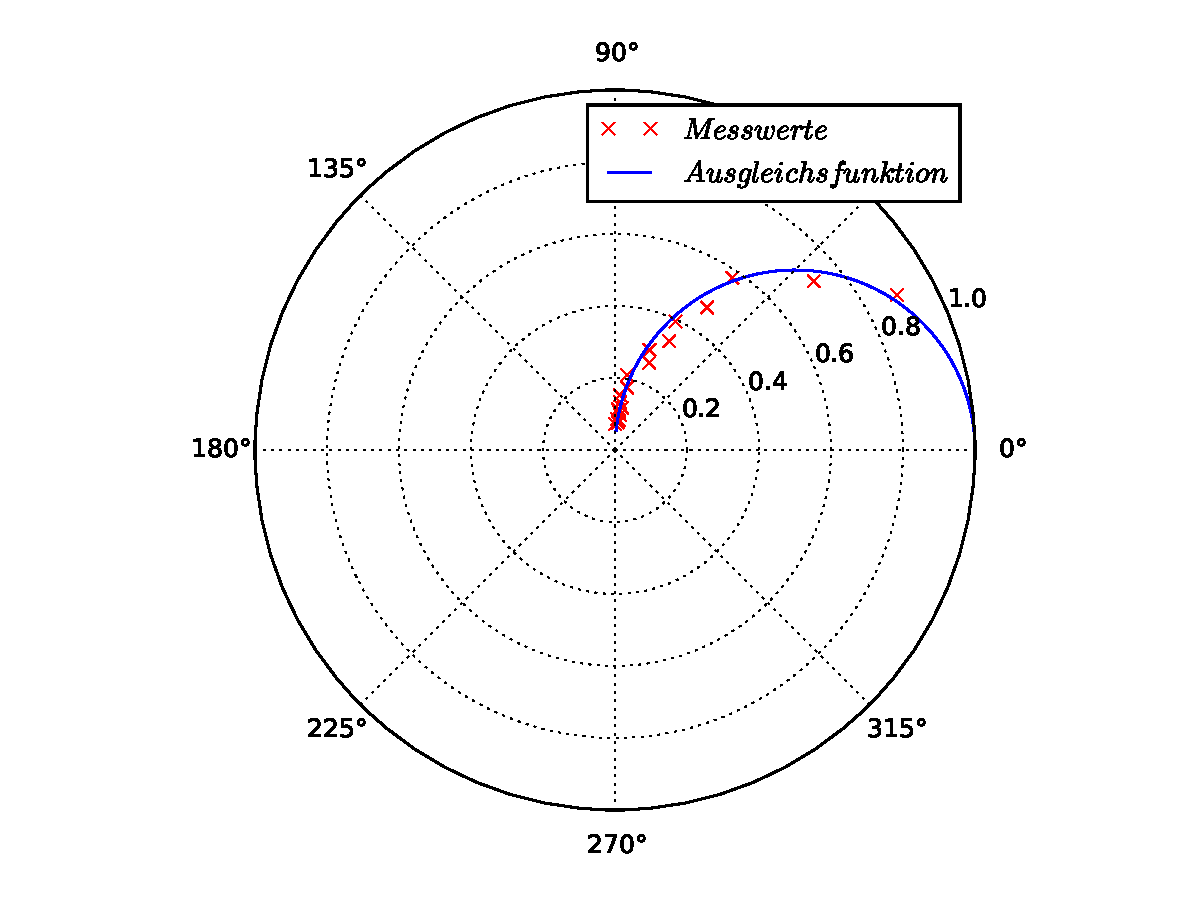
\includegraphics[width=0.8\textwidth]{d.pdf}
\caption{Amplitude $A_0$ in Abbhängigkeit von der Phasenverschiebung $\phi$ }
\label{abb:d}
\end{figure}
\FloatBarrier
\subsection{Eignung als Integrator}
Die folgenden Abbildungen zeigen die integrierten Kurven von Dreiecks-,Rechtsecks-und Sinusspannung.
Für eine Phase Sinusspannung, ergibt sich, wie in Abbildung \ref{abb:sinus} zu sehen, eine Cosinusspannung, dies entspricht auch der Stammfunktion:
\begin{align}
  f(x)&=a\cdot \sin{x}&F(x)&=-a\cdot \cos{x}.
\end{align}\\
Bei einer Phase der Rechtecksspannung ergibt sich als integrierte Spannung eine Grade mit konstanter Steigung,
zu erkennen anhand der Abbildung \ref{abb:rechteck} und der Stammfunktion:
\begin{align}
  f(x)=
  \begin{cases}
    a,& 0 \leq t \textless \pi\\
   -a,& -\pi \leq t \textless 0
  \end{cases}
  \ \ \ \ \ \ \ \ \
  F(x)=
  \begin{cases}
    a\cdot x,& 0 \leq t \textless \pi\\
   -a\cdot x,&  -\pi \leq t \textless 0.
  \end{cases}
\end{align}\\
Für eine Phase der Dreiecksspannung ergibt sich als integrierte Spannung eine Parabel, dies ist sowohl in Abbildung \ref{abb:dreieck} als auch anhand der Stammfunktion zu erkennen:
\begin{align}
  f(x)=
  \begin{cases}
    a\cdot x,& 0 \leq t \textless \pi\\
   -a\cdot x,&  -\pi \leq t \textless 0
  \end{cases}
  \ \ \ \ \ \ \ \ \
  F(x)=
  \begin{cases}
    \frac{a}{2}\cdot x^2,& 0 \leq t \textless \pi\\
   \frac{-a}{2}\cdot x^2,&  -\pi \leq t \textless 0.
  \end{cases}
\end{align}\\
\begin{figure}[h]
    \centering
    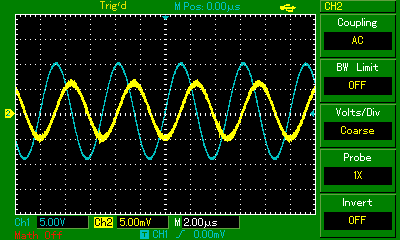
\includegraphics[width=0.6\textwidth]{MAP007.png}
    \caption{Bild der Sinusspannung und ihrer Integrierten Spannung.}
    \label{abb:sinus}
\end{figure}\\
\begin{figure}[h]
    \centering
    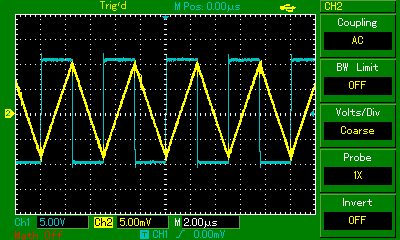
\includegraphics[width=0.6\textwidth]{MAP006.png}
    \caption{Bild der Rechteckspannung und ihrer Integrierten Spannung.}
    \label{abb:rechteck}
\end{figure}\\
\begin{figure}[h]
    \centering
    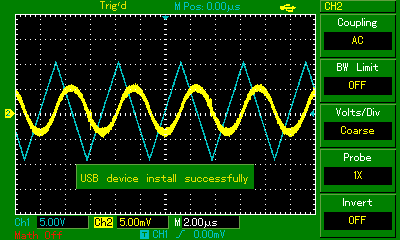
\includegraphics[width=0.6\textwidth]{MAP005.png}
    \caption{Bild der Dreicksspannung und ihrer Integrierten Spannung.}
    \label{abb:dreieck}
\end{figure}\\

\section{Diskussion}
\label{sec:Diskussion}
Nun werden die aus der Auswertung erhaltenen
Ergebnisse in Hinblick auf die Theorie untersucht.
Zu einem muss gesagt werden das die Messwerte aus der Abbildung \ref{abb:c} stark
um die Ausgleichsfunktion streuen, dies liegt daran das die Zeitabstände a und b mit
Hilfe der Cursers des Oszilloskopes gemesssen wurde und diese nicht genau eingestellt werden konnten.
Dies ließe sich mit einem Oszilloskop, das die Daten speichert und ausgibt verhmeiden.
Ebenfalls würde mit Erhöhung der Messpaare im niedrigerem Frequenzbereich die Zeitkonstant $RC$ genauer werden .
Außerdem wurde eine Frequenzabhängigkeit bei der Spannung $U_0$ gemessen, diese sank bei höheren Frequenzen ab.
Diese ist aber für den Frequenzbreich, indem die Messungen durchgeführt
worden sind, sehr gering und kann somit vernachlässigt werden.
Die bei den anderen Messverfahren erhaltenen Ergebnisse bestätigen
die aus dem Kapitel \ref{sec:Theorie} aufgeführten Formeln.


\printbibliography

\end{document}
>>>>>>> theorie und durchführung
